\chapter{Overview of the Company}
\section{History of the Organization }
DCSELab (National key Laboratory of Digital Control and System Engineering), founded on 04/08/2003 under Decision number 590/QD/DHQG/TCCB of Vietnam National Unversity Ho Chi Minh City. It is an independent organization which has a status of legal person; conducts technological advancement on its own accord based on the Regulation for developing and functioning of National key Laboratory.
\begin{figure}[h]
	\centering
	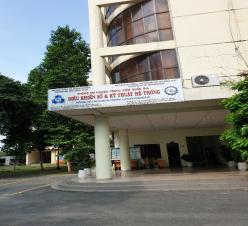
\includegraphics{01}
	\caption{DCSELab main entrance}
	\label{fig:01}
\end{figure}
\section{Working Objectives}
Experimenting, designing, installing, maintaining and transferring equipment (hardware and software) regarding digital control, system engineering; mechatronics, telecommunication, information technology, automation and industrial process.
\section{The Organizational Structure}
\begin{figure}[ht]
	\centering
	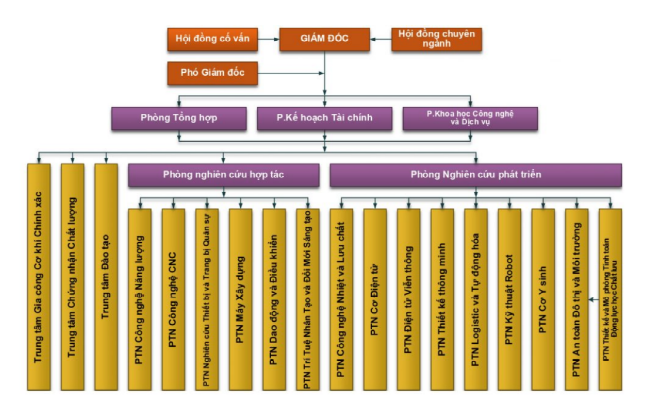
\includegraphics{02}
	\caption{The organizational structure of DCSELab}
	\label{fig:02}
\end{figure}
